
\begin{figure}
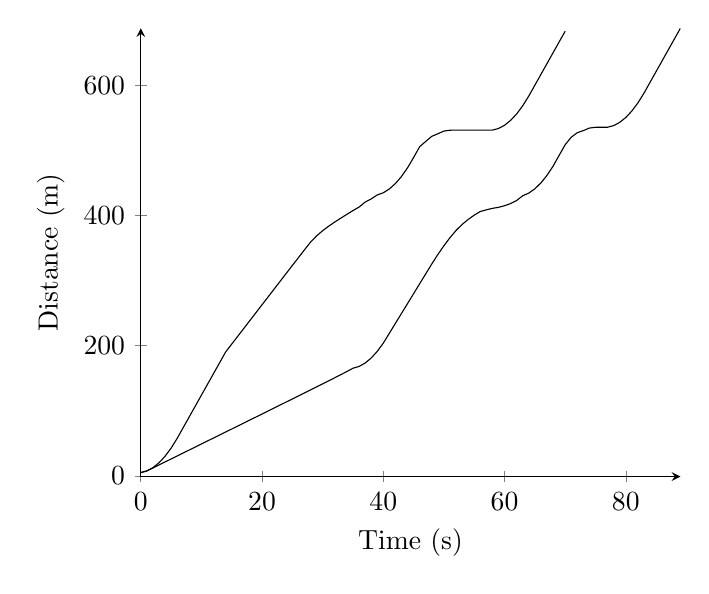
\begin{tikzpicture}
\begin{axis}[
legend style={anchor=west},
axis x line=bottom,
axis y line=left,
ymin=-1,
xlabel=Time (s),
ylabel=Distance (m),
]
\addplot[] coordinates {
(0, 5.1)
(1, 7.6)
(2, 12.6)
(3, 20.1)
(4, 30.1)
(5, 42.6)
(6, 57.6)
(7, 74.2)
(8, 90.8)
(9, 107.4)
(10, 124.0)
(11, 140.6)
(12, 157.2)
(13, 173.8)
(14, 190.4)
(15, 202.485060286)
(16, 214.570153993)
(17, 226.655286686)
(18, 238.740465238)
(19, 250.825698238)
(20, 262.910996565)
(21, 274.996374199)
(22, 287.08184942)
(23, 299.167446592)
(24, 311.253198924)
(25, 323.339152889)
(26, 335.28537558)
(27, 347.371874288)
(28, 359.174264817)
(29, 368.736704215)
(30, 376.756942552)
(31, 383.738518487)
(32, 390.082397681)
(33, 396.073194509)
(34, 401.892669859)
(35, 407.663511614)
(36, 413.008615805)
(37, 420.668063263)
(38, 425.542870423)
(39, 431.670201805)
(40, 435.016729414)
(41, 440.863257022)
(42, 449.209784631)
(43, 460.056312239)
(44, 473.402839848)
(45, 489.249367456)
(46, 505.849367456)
(47, 513.895787708)
(48, 521.767000615)
(49, 525.664272594)
(50, 529.820488861)
(51, 531.119402045)
(52, 531.258390191)
(53, 531.258390191)
(54, 531.258390191)
(55, 531.258390191)
(56, 531.258390191)
(57, 531.258390191)
(58, 531.258390191)
(59, 533.758390191)
(60, 538.758390191)
(61, 546.258390191)
(62, 556.258390191)
(63, 568.758390191)
(64, 583.758390191)
(65, 600.358390191)
(66, 616.958390191)
(67, 633.558390191)
(68, 650.158390191)
(69, 666.758390191)
(70, 683.358390191)
};
\addplot[] coordinates {
(0, 5.1)
(1, 7.6)
(2, 12.1993814825)
(3, 16.799045433)
(4, 21.3990159658)
(5, 25.9993200238)
(6, 30.5999878064)
(7, 35.2010532776)
(8, 39.8025547724)
(9, 44.4045357245)
(10, 49.0070455444)
(11, 53.6101406867)
(12, 58.2138859536)
(13, 62.8183561014)
(14, 67.4236378321)
(15, 72.0298322858)
(16, 76.6370581851)
(17, 81.2454558427)
(18, 85.8551923199)
(19, 90.4664681464)
(20, 95.0795261806)
(21, 99.6946634582)
(22, 104.312247279)
(23, 108.932737428)
(24, 113.556717463)
(25, 118.184939739)
(26, 122.818391849)
(27, 127.452495438)
(28, 132.094863979)
(29, 136.748197731)
(30, 141.416274366)
(31, 146.104886951)
(32, 150.823453364)
(33, 155.588555598)
(34, 160.433025922)
(35, 165.435918862)
(36, 168.147346624)
(37, 173.358774387)
(38, 181.070202149)
(39, 191.281629912)
(40, 203.993057674)
(41, 219.200107328)
(42, 234.407221754)
(43, 249.614416032)
(44, 264.821710316)
(45, 280.036049923)
(46, 295.251266857)
(47, 310.467657214)
(48, 325.685667143)
(49, 340.206931855)
(50, 353.694842028)
(51, 366.077034013)
(52, 377.143314312)
(53, 386.325564424)
(54, 393.995541488)
(55, 400.633266302)
(56, 406.231949097)
(57, 408.835239795)
(58, 411.065293463)
(59, 412.612886983)
(60, 415.129775062)
(61, 418.444107034)
(62, 423.206663542)
(63, 430.46922005)
(64, 434.557300115)
(65, 441.14538018)
(66, 450.233460245)
(67, 461.82154031)
(68, 475.909620375)
(69, 492.49770044)
(70, 508.918842131)
(71, 520.401802247)
(72, 527.357819113)
(73, 530.544013681)
(74, 534.449155569)
(75, 535.608075402)
(76, 535.718975105)
(77, 535.718975105)
(78, 538.218975105)
(79, 543.218975105)
(80, 550.718975105)
(81, 560.718975105)
(82, 573.218975105)
(83, 588.218975105)
(84, 604.818975105)
(85, 621.418975105)
(86, 638.018975105)
(87, 654.618975105)
(88, 671.218975105)
(89, 687.818975105)
};

\end{axis}
\end{tikzpicture}
\label{tik:100:79}
\caption{100 percent diving with GSC on route $79$}
\end{figure}
